% Created by tikzDevice version 0.12.3.1 on 2022-03-28 12:19:50
% !TEX encoding = UTF-8 Unicode
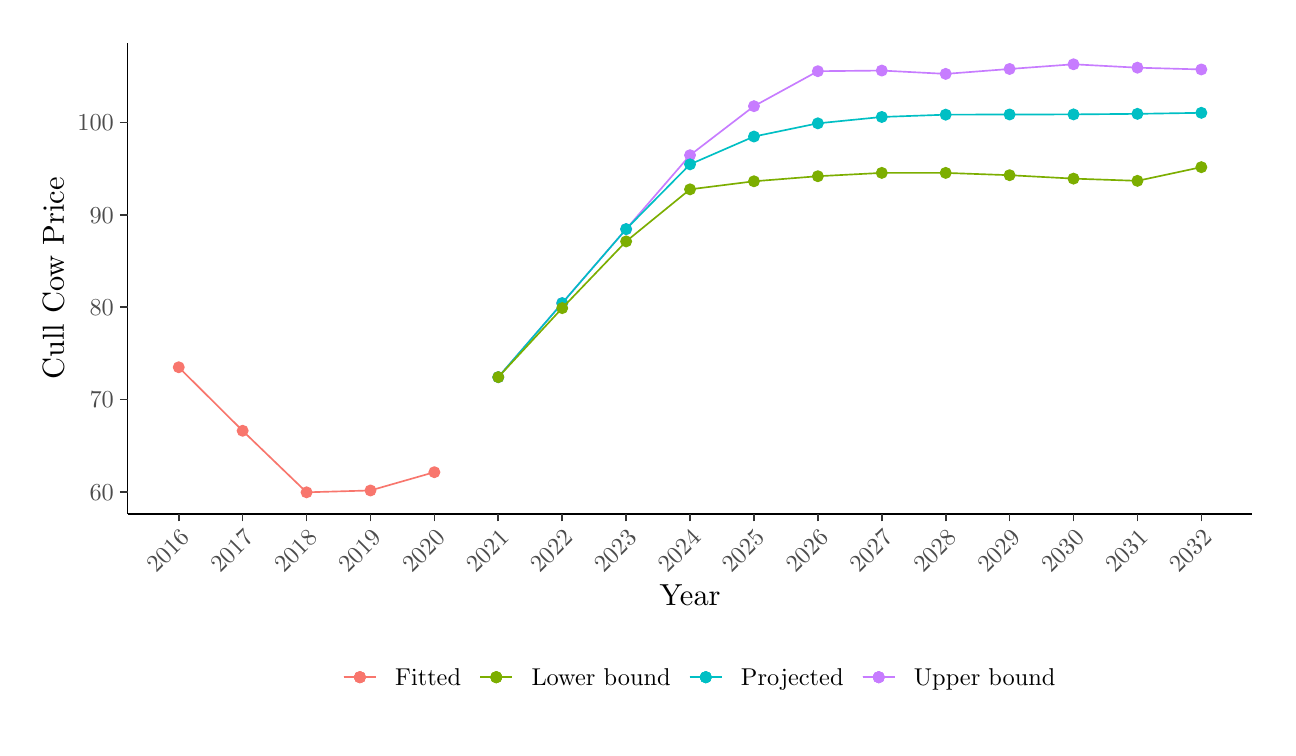
\begin{tikzpicture}[x=1pt,y=1pt]
\definecolor{fillColor}{RGB}{255,255,255}
\path[use as bounding box,fill=fillColor,fill opacity=0.00] (0,0) rectangle (448.07,252.94);
\begin{scope}
\path[clip] (  0.00,  0.00) rectangle (448.07,252.94);
\definecolor{drawColor}{RGB}{255,255,255}
\definecolor{fillColor}{RGB}{255,255,255}

\path[draw=drawColor,line width= 0.6pt,line join=round,line cap=round,fill=fillColor] (  0.00,  0.00) rectangle (448.07,252.94);
\end{scope}
\begin{scope}
\path[clip] ( 36.11, 77.31) rectangle (442.57,247.44);
\definecolor{fillColor}{RGB}{255,255,255}

\path[fill=fillColor] ( 36.11, 77.31) rectangle (442.57,247.44);
\definecolor{drawColor}{RGB}{248,118,109}

\path[draw=drawColor,line width= 0.6pt,line join=round] ( 54.59,130.23) --
	( 77.68,107.28) --
	(100.78, 85.04) --
	(123.87, 85.71) --
	(146.96, 92.31);
\definecolor{fillColor}{RGB}{248,118,109}

\path[draw=drawColor,line width= 0.4pt,line join=round,line cap=round,fill=fillColor] ( 54.59,130.23) circle (  1.96);

\path[draw=drawColor,line width= 0.4pt,line join=round,line cap=round,fill=fillColor] ( 77.68,107.28) circle (  1.96);

\path[draw=drawColor,line width= 0.4pt,line join=round,line cap=round,fill=fillColor] (100.78, 85.04) circle (  1.96);

\path[draw=drawColor,line width= 0.4pt,line join=round,line cap=round,fill=fillColor] (123.87, 85.71) circle (  1.96);

\path[draw=drawColor,line width= 0.4pt,line join=round,line cap=round,fill=fillColor] (146.96, 92.31) circle (  1.96);
\definecolor{drawColor}{RGB}{199,124,255}

\path[draw=drawColor,line width= 0.6pt,line join=round] (170.06,126.66) --
	(193.15,153.40) --
	(216.25,180.15) --
	(239.34,206.86) --
	(262.44,224.57) --
	(285.53,237.21) --
	(308.63,237.44) --
	(331.72,236.24) --
	(354.81,238.01) --
	(377.91,239.71) --
	(401.00,238.48) --
	(424.10,237.84);
\definecolor{fillColor}{RGB}{199,124,255}

\path[draw=drawColor,line width= 0.4pt,line join=round,line cap=round,fill=fillColor] (170.06,126.66) circle (  1.96);

\path[draw=drawColor,line width= 0.4pt,line join=round,line cap=round,fill=fillColor] (193.15,153.40) circle (  1.96);

\path[draw=drawColor,line width= 0.4pt,line join=round,line cap=round,fill=fillColor] (216.25,180.15) circle (  1.96);

\path[draw=drawColor,line width= 0.4pt,line join=round,line cap=round,fill=fillColor] (239.34,206.86) circle (  1.96);

\path[draw=drawColor,line width= 0.4pt,line join=round,line cap=round,fill=fillColor] (262.44,224.57) circle (  1.96);

\path[draw=drawColor,line width= 0.4pt,line join=round,line cap=round,fill=fillColor] (285.53,237.21) circle (  1.96);

\path[draw=drawColor,line width= 0.4pt,line join=round,line cap=round,fill=fillColor] (308.63,237.44) circle (  1.96);

\path[draw=drawColor,line width= 0.4pt,line join=round,line cap=round,fill=fillColor] (331.72,236.24) circle (  1.96);

\path[draw=drawColor,line width= 0.4pt,line join=round,line cap=round,fill=fillColor] (354.81,238.01) circle (  1.96);

\path[draw=drawColor,line width= 0.4pt,line join=round,line cap=round,fill=fillColor] (377.91,239.71) circle (  1.96);

\path[draw=drawColor,line width= 0.4pt,line join=round,line cap=round,fill=fillColor] (401.00,238.48) circle (  1.96);

\path[draw=drawColor,line width= 0.4pt,line join=round,line cap=round,fill=fillColor] (424.10,237.84) circle (  1.96);
\definecolor{drawColor}{RGB}{0,191,196}

\path[draw=drawColor,line width= 0.6pt,line join=round] (170.06,126.66) --
	(193.15,153.40) --
	(216.25,180.15) --
	(239.34,203.56) --
	(262.44,213.60) --
	(285.53,218.37) --
	(308.63,220.67) --
	(331.72,221.50) --
	(354.81,221.57) --
	(377.91,221.60) --
	(401.00,221.80) --
	(424.10,222.17);
\definecolor{fillColor}{RGB}{0,191,196}

\path[draw=drawColor,line width= 0.4pt,line join=round,line cap=round,fill=fillColor] (170.06,126.66) circle (  1.96);

\path[draw=drawColor,line width= 0.4pt,line join=round,line cap=round,fill=fillColor] (193.15,153.40) circle (  1.96);

\path[draw=drawColor,line width= 0.4pt,line join=round,line cap=round,fill=fillColor] (216.25,180.15) circle (  1.96);

\path[draw=drawColor,line width= 0.4pt,line join=round,line cap=round,fill=fillColor] (239.34,203.56) circle (  1.96);

\path[draw=drawColor,line width= 0.4pt,line join=round,line cap=round,fill=fillColor] (262.44,213.60) circle (  1.96);

\path[draw=drawColor,line width= 0.4pt,line join=round,line cap=round,fill=fillColor] (285.53,218.37) circle (  1.96);

\path[draw=drawColor,line width= 0.4pt,line join=round,line cap=round,fill=fillColor] (308.63,220.67) circle (  1.96);

\path[draw=drawColor,line width= 0.4pt,line join=round,line cap=round,fill=fillColor] (331.72,221.50) circle (  1.96);

\path[draw=drawColor,line width= 0.4pt,line join=round,line cap=round,fill=fillColor] (354.81,221.57) circle (  1.96);

\path[draw=drawColor,line width= 0.4pt,line join=round,line cap=round,fill=fillColor] (377.91,221.60) circle (  1.96);

\path[draw=drawColor,line width= 0.4pt,line join=round,line cap=round,fill=fillColor] (401.00,221.80) circle (  1.96);

\path[draw=drawColor,line width= 0.4pt,line join=round,line cap=round,fill=fillColor] (424.10,222.17) circle (  1.96);
\definecolor{drawColor}{RGB}{124,174,0}

\path[draw=drawColor,line width= 0.6pt,line join=round] (170.06,126.66) --
	(193.15,151.60) --
	(216.25,175.71) --
	(239.34,194.52) --
	(262.44,197.43) --
	(285.53,199.26) --
	(308.63,200.46) --
	(331.72,200.46) --
	(354.81,199.63) --
	(377.91,198.39) --
	(401.00,197.59) --
	(424.10,202.53);
\definecolor{fillColor}{RGB}{124,174,0}

\path[draw=drawColor,line width= 0.4pt,line join=round,line cap=round,fill=fillColor] (170.06,126.66) circle (  1.96);

\path[draw=drawColor,line width= 0.4pt,line join=round,line cap=round,fill=fillColor] (193.15,151.60) circle (  1.96);

\path[draw=drawColor,line width= 0.4pt,line join=round,line cap=round,fill=fillColor] (216.25,175.71) circle (  1.96);

\path[draw=drawColor,line width= 0.4pt,line join=round,line cap=round,fill=fillColor] (239.34,194.52) circle (  1.96);

\path[draw=drawColor,line width= 0.4pt,line join=round,line cap=round,fill=fillColor] (262.44,197.43) circle (  1.96);

\path[draw=drawColor,line width= 0.4pt,line join=round,line cap=round,fill=fillColor] (285.53,199.26) circle (  1.96);

\path[draw=drawColor,line width= 0.4pt,line join=round,line cap=round,fill=fillColor] (308.63,200.46) circle (  1.96);

\path[draw=drawColor,line width= 0.4pt,line join=round,line cap=round,fill=fillColor] (331.72,200.46) circle (  1.96);

\path[draw=drawColor,line width= 0.4pt,line join=round,line cap=round,fill=fillColor] (354.81,199.63) circle (  1.96);

\path[draw=drawColor,line width= 0.4pt,line join=round,line cap=round,fill=fillColor] (377.91,198.39) circle (  1.96);

\path[draw=drawColor,line width= 0.4pt,line join=round,line cap=round,fill=fillColor] (401.00,197.59) circle (  1.96);

\path[draw=drawColor,line width= 0.4pt,line join=round,line cap=round,fill=fillColor] (424.10,202.53) circle (  1.96);
\end{scope}
\begin{scope}
\path[clip] (  0.00,  0.00) rectangle (448.07,252.94);
\definecolor{drawColor}{RGB}{0,0,0}

\path[draw=drawColor,line width= 0.6pt,line join=round] ( 36.11, 77.31) --
	( 36.11,247.44);
\end{scope}
\begin{scope}
\path[clip] (  0.00,  0.00) rectangle (448.07,252.94);
\definecolor{drawColor}{gray}{0.30}

\node[text=drawColor,anchor=base east,inner sep=0pt, outer sep=0pt, scale=  0.88] at ( 31.16, 82.24) {60};

\node[text=drawColor,anchor=base east,inner sep=0pt, outer sep=0pt, scale=  0.88] at ( 31.16,115.59) {70};

\node[text=drawColor,anchor=base east,inner sep=0pt, outer sep=0pt, scale=  0.88] at ( 31.16,148.94) {80};

\node[text=drawColor,anchor=base east,inner sep=0pt, outer sep=0pt, scale=  0.88] at ( 31.16,182.29) {90};

\node[text=drawColor,anchor=base east,inner sep=0pt, outer sep=0pt, scale=  0.88] at ( 31.16,215.64) {100};
\end{scope}
\begin{scope}
\path[clip] (  0.00,  0.00) rectangle (448.07,252.94);
\definecolor{drawColor}{gray}{0.20}

\path[draw=drawColor,line width= 0.6pt,line join=round] ( 33.36, 85.27) --
	( 36.11, 85.27);

\path[draw=drawColor,line width= 0.6pt,line join=round] ( 33.36,118.62) --
	( 36.11,118.62);

\path[draw=drawColor,line width= 0.6pt,line join=round] ( 33.36,151.97) --
	( 36.11,151.97);

\path[draw=drawColor,line width= 0.6pt,line join=round] ( 33.36,185.32) --
	( 36.11,185.32);

\path[draw=drawColor,line width= 0.6pt,line join=round] ( 33.36,218.67) --
	( 36.11,218.67);
\end{scope}
\begin{scope}
\path[clip] (  0.00,  0.00) rectangle (448.07,252.94);
\definecolor{drawColor}{RGB}{0,0,0}

\path[draw=drawColor,line width= 0.6pt,line join=round] ( 36.11, 77.31) --
	(442.57, 77.31);
\end{scope}
\begin{scope}
\path[clip] (  0.00,  0.00) rectangle (448.07,252.94);
\definecolor{drawColor}{gray}{0.20}

\path[draw=drawColor,line width= 0.6pt,line join=round] ( 54.59, 74.56) --
	( 54.59, 77.31);

\path[draw=drawColor,line width= 0.6pt,line join=round] ( 77.68, 74.56) --
	( 77.68, 77.31);

\path[draw=drawColor,line width= 0.6pt,line join=round] (100.78, 74.56) --
	(100.78, 77.31);

\path[draw=drawColor,line width= 0.6pt,line join=round] (123.87, 74.56) --
	(123.87, 77.31);

\path[draw=drawColor,line width= 0.6pt,line join=round] (146.96, 74.56) --
	(146.96, 77.31);

\path[draw=drawColor,line width= 0.6pt,line join=round] (170.06, 74.56) --
	(170.06, 77.31);

\path[draw=drawColor,line width= 0.6pt,line join=round] (193.15, 74.56) --
	(193.15, 77.31);

\path[draw=drawColor,line width= 0.6pt,line join=round] (216.25, 74.56) --
	(216.25, 77.31);

\path[draw=drawColor,line width= 0.6pt,line join=round] (239.34, 74.56) --
	(239.34, 77.31);

\path[draw=drawColor,line width= 0.6pt,line join=round] (262.44, 74.56) --
	(262.44, 77.31);

\path[draw=drawColor,line width= 0.6pt,line join=round] (285.53, 74.56) --
	(285.53, 77.31);

\path[draw=drawColor,line width= 0.6pt,line join=round] (308.63, 74.56) --
	(308.63, 77.31);

\path[draw=drawColor,line width= 0.6pt,line join=round] (331.72, 74.56) --
	(331.72, 77.31);

\path[draw=drawColor,line width= 0.6pt,line join=round] (354.81, 74.56) --
	(354.81, 77.31);

\path[draw=drawColor,line width= 0.6pt,line join=round] (377.91, 74.56) --
	(377.91, 77.31);

\path[draw=drawColor,line width= 0.6pt,line join=round] (401.00, 74.56) --
	(401.00, 77.31);

\path[draw=drawColor,line width= 0.6pt,line join=round] (424.10, 74.56) --
	(424.10, 77.31);
\end{scope}
\begin{scope}
\path[clip] (  0.00,  0.00) rectangle (448.07,252.94);
\definecolor{drawColor}{gray}{0.30}

\node[text=drawColor,rotate= 45.00,anchor=base east,inner sep=0pt, outer sep=0pt, scale=  0.88] at ( 58.87, 68.07) {2016};

\node[text=drawColor,rotate= 45.00,anchor=base east,inner sep=0pt, outer sep=0pt, scale=  0.88] at ( 81.97, 68.07) {2017};

\node[text=drawColor,rotate= 45.00,anchor=base east,inner sep=0pt, outer sep=0pt, scale=  0.88] at (105.06, 68.07) {2018};

\node[text=drawColor,rotate= 45.00,anchor=base east,inner sep=0pt, outer sep=0pt, scale=  0.88] at (128.16, 68.07) {2019};

\node[text=drawColor,rotate= 45.00,anchor=base east,inner sep=0pt, outer sep=0pt, scale=  0.88] at (151.25, 68.07) {2020};

\node[text=drawColor,rotate= 45.00,anchor=base east,inner sep=0pt, outer sep=0pt, scale=  0.88] at (174.34, 68.07) {2021};

\node[text=drawColor,rotate= 45.00,anchor=base east,inner sep=0pt, outer sep=0pt, scale=  0.88] at (197.44, 68.07) {2022};

\node[text=drawColor,rotate= 45.00,anchor=base east,inner sep=0pt, outer sep=0pt, scale=  0.88] at (220.53, 68.07) {2023};

\node[text=drawColor,rotate= 45.00,anchor=base east,inner sep=0pt, outer sep=0pt, scale=  0.88] at (243.63, 68.07) {2024};

\node[text=drawColor,rotate= 45.00,anchor=base east,inner sep=0pt, outer sep=0pt, scale=  0.88] at (266.72, 68.07) {2025};

\node[text=drawColor,rotate= 45.00,anchor=base east,inner sep=0pt, outer sep=0pt, scale=  0.88] at (289.82, 68.07) {2026};

\node[text=drawColor,rotate= 45.00,anchor=base east,inner sep=0pt, outer sep=0pt, scale=  0.88] at (312.91, 68.07) {2027};

\node[text=drawColor,rotate= 45.00,anchor=base east,inner sep=0pt, outer sep=0pt, scale=  0.88] at (336.01, 68.07) {2028};

\node[text=drawColor,rotate= 45.00,anchor=base east,inner sep=0pt, outer sep=0pt, scale=  0.88] at (359.10, 68.07) {2029};

\node[text=drawColor,rotate= 45.00,anchor=base east,inner sep=0pt, outer sep=0pt, scale=  0.88] at (382.20, 68.07) {2030};

\node[text=drawColor,rotate= 45.00,anchor=base east,inner sep=0pt, outer sep=0pt, scale=  0.88] at (405.29, 68.07) {2031};

\node[text=drawColor,rotate= 45.00,anchor=base east,inner sep=0pt, outer sep=0pt, scale=  0.88] at (428.38, 68.07) {2032};
\end{scope}
\begin{scope}
\path[clip] (  0.00,  0.00) rectangle (448.07,252.94);
\definecolor{drawColor}{RGB}{0,0,0}

\node[text=drawColor,anchor=base,inner sep=0pt, outer sep=0pt, scale=  1.10] at (239.34, 44.09) {Year};
\end{scope}
\begin{scope}
\path[clip] (  0.00,  0.00) rectangle (448.07,252.94);
\definecolor{drawColor}{RGB}{0,0,0}

\node[text=drawColor,rotate= 90.00,anchor=base,inner sep=0pt, outer sep=0pt, scale=  1.10] at ( 13.08,162.38) {Cull Cow Price};
\end{scope}
\begin{scope}
\path[clip] (  0.00,  0.00) rectangle (448.07,252.94);
\definecolor{fillColor}{RGB}{255,255,255}

\path[fill=fillColor] (101.82,  5.50) rectangle (376.86, 30.95);
\end{scope}
\begin{scope}
\path[clip] (  0.00,  0.00) rectangle (448.07,252.94);
\definecolor{drawColor}{RGB}{248,118,109}

\path[draw=drawColor,line width= 0.6pt,line join=round] (114.27, 18.23) -- (125.83, 18.23);
\end{scope}
\begin{scope}
\path[clip] (  0.00,  0.00) rectangle (448.07,252.94);
\definecolor{drawColor}{RGB}{248,118,109}
\definecolor{fillColor}{RGB}{248,118,109}

\path[draw=drawColor,line width= 0.4pt,line join=round,line cap=round,fill=fillColor] (120.05, 18.23) circle (  1.96);
\end{scope}
\begin{scope}
\path[clip] (  0.00,  0.00) rectangle (448.07,252.94);
\definecolor{drawColor}{RGB}{248,118,109}

\path[draw=drawColor,line width= 0.6pt,line join=round] (114.27, 18.23) -- (125.83, 18.23);
\end{scope}
\begin{scope}
\path[clip] (  0.00,  0.00) rectangle (448.07,252.94);
\definecolor{drawColor}{RGB}{248,118,109}
\definecolor{fillColor}{RGB}{248,118,109}

\path[draw=drawColor,line width= 0.4pt,line join=round,line cap=round,fill=fillColor] (120.05, 18.23) circle (  1.96);
\end{scope}
\begin{scope}
\path[clip] (  0.00,  0.00) rectangle (448.07,252.94);
\definecolor{drawColor}{RGB}{248,118,109}

\path[draw=drawColor,line width= 0.6pt,line join=round] (114.27, 18.23) -- (125.83, 18.23);
\end{scope}
\begin{scope}
\path[clip] (  0.00,  0.00) rectangle (448.07,252.94);
\definecolor{drawColor}{RGB}{248,118,109}
\definecolor{fillColor}{RGB}{248,118,109}

\path[draw=drawColor,line width= 0.4pt,line join=round,line cap=round,fill=fillColor] (120.05, 18.23) circle (  1.96);
\end{scope}
\begin{scope}
\path[clip] (  0.00,  0.00) rectangle (448.07,252.94);
\definecolor{drawColor}{RGB}{248,118,109}

\path[draw=drawColor,line width= 0.6pt,line join=round] (114.27, 18.23) -- (125.83, 18.23);
\end{scope}
\begin{scope}
\path[clip] (  0.00,  0.00) rectangle (448.07,252.94);
\definecolor{drawColor}{RGB}{248,118,109}
\definecolor{fillColor}{RGB}{248,118,109}

\path[draw=drawColor,line width= 0.4pt,line join=round,line cap=round,fill=fillColor] (120.05, 18.23) circle (  1.96);
\end{scope}
\begin{scope}
\path[clip] (  0.00,  0.00) rectangle (448.07,252.94);
\definecolor{drawColor}{RGB}{124,174,0}

\path[draw=drawColor,line width= 0.6pt,line join=round] (163.55, 18.23) -- (175.11, 18.23);
\end{scope}
\begin{scope}
\path[clip] (  0.00,  0.00) rectangle (448.07,252.94);
\definecolor{drawColor}{RGB}{124,174,0}
\definecolor{fillColor}{RGB}{124,174,0}

\path[draw=drawColor,line width= 0.4pt,line join=round,line cap=round,fill=fillColor] (169.33, 18.23) circle (  1.96);
\end{scope}
\begin{scope}
\path[clip] (  0.00,  0.00) rectangle (448.07,252.94);
\definecolor{drawColor}{RGB}{124,174,0}

\path[draw=drawColor,line width= 0.6pt,line join=round] (163.55, 18.23) -- (175.11, 18.23);
\end{scope}
\begin{scope}
\path[clip] (  0.00,  0.00) rectangle (448.07,252.94);
\definecolor{drawColor}{RGB}{124,174,0}
\definecolor{fillColor}{RGB}{124,174,0}

\path[draw=drawColor,line width= 0.4pt,line join=round,line cap=round,fill=fillColor] (169.33, 18.23) circle (  1.96);
\end{scope}
\begin{scope}
\path[clip] (  0.00,  0.00) rectangle (448.07,252.94);
\definecolor{drawColor}{RGB}{124,174,0}

\path[draw=drawColor,line width= 0.6pt,line join=round] (163.55, 18.23) -- (175.11, 18.23);
\end{scope}
\begin{scope}
\path[clip] (  0.00,  0.00) rectangle (448.07,252.94);
\definecolor{drawColor}{RGB}{124,174,0}
\definecolor{fillColor}{RGB}{124,174,0}

\path[draw=drawColor,line width= 0.4pt,line join=round,line cap=round,fill=fillColor] (169.33, 18.23) circle (  1.96);
\end{scope}
\begin{scope}
\path[clip] (  0.00,  0.00) rectangle (448.07,252.94);
\definecolor{drawColor}{RGB}{124,174,0}

\path[draw=drawColor,line width= 0.6pt,line join=round] (163.55, 18.23) -- (175.11, 18.23);
\end{scope}
\begin{scope}
\path[clip] (  0.00,  0.00) rectangle (448.07,252.94);
\definecolor{drawColor}{RGB}{124,174,0}
\definecolor{fillColor}{RGB}{124,174,0}

\path[draw=drawColor,line width= 0.4pt,line join=round,line cap=round,fill=fillColor] (169.33, 18.23) circle (  1.96);
\end{scope}
\begin{scope}
\path[clip] (  0.00,  0.00) rectangle (448.07,252.94);
\definecolor{drawColor}{RGB}{0,191,196}

\path[draw=drawColor,line width= 0.6pt,line join=round] (239.25, 18.23) -- (250.81, 18.23);
\end{scope}
\begin{scope}
\path[clip] (  0.00,  0.00) rectangle (448.07,252.94);
\definecolor{drawColor}{RGB}{0,191,196}
\definecolor{fillColor}{RGB}{0,191,196}

\path[draw=drawColor,line width= 0.4pt,line join=round,line cap=round,fill=fillColor] (245.03, 18.23) circle (  1.96);
\end{scope}
\begin{scope}
\path[clip] (  0.00,  0.00) rectangle (448.07,252.94);
\definecolor{drawColor}{RGB}{0,191,196}

\path[draw=drawColor,line width= 0.6pt,line join=round] (239.25, 18.23) -- (250.81, 18.23);
\end{scope}
\begin{scope}
\path[clip] (  0.00,  0.00) rectangle (448.07,252.94);
\definecolor{drawColor}{RGB}{0,191,196}
\definecolor{fillColor}{RGB}{0,191,196}

\path[draw=drawColor,line width= 0.4pt,line join=round,line cap=round,fill=fillColor] (245.03, 18.23) circle (  1.96);
\end{scope}
\begin{scope}
\path[clip] (  0.00,  0.00) rectangle (448.07,252.94);
\definecolor{drawColor}{RGB}{0,191,196}

\path[draw=drawColor,line width= 0.6pt,line join=round] (239.25, 18.23) -- (250.81, 18.23);
\end{scope}
\begin{scope}
\path[clip] (  0.00,  0.00) rectangle (448.07,252.94);
\definecolor{drawColor}{RGB}{0,191,196}
\definecolor{fillColor}{RGB}{0,191,196}

\path[draw=drawColor,line width= 0.4pt,line join=round,line cap=round,fill=fillColor] (245.03, 18.23) circle (  1.96);
\end{scope}
\begin{scope}
\path[clip] (  0.00,  0.00) rectangle (448.07,252.94);
\definecolor{drawColor}{RGB}{0,191,196}

\path[draw=drawColor,line width= 0.6pt,line join=round] (239.25, 18.23) -- (250.81, 18.23);
\end{scope}
\begin{scope}
\path[clip] (  0.00,  0.00) rectangle (448.07,252.94);
\definecolor{drawColor}{RGB}{0,191,196}
\definecolor{fillColor}{RGB}{0,191,196}

\path[draw=drawColor,line width= 0.4pt,line join=round,line cap=round,fill=fillColor] (245.03, 18.23) circle (  1.96);
\end{scope}
\begin{scope}
\path[clip] (  0.00,  0.00) rectangle (448.07,252.94);
\definecolor{drawColor}{RGB}{199,124,255}

\path[draw=drawColor,line width= 0.6pt,line join=round] (301.75, 18.23) -- (313.32, 18.23);
\end{scope}
\begin{scope}
\path[clip] (  0.00,  0.00) rectangle (448.07,252.94);
\definecolor{drawColor}{RGB}{199,124,255}
\definecolor{fillColor}{RGB}{199,124,255}

\path[draw=drawColor,line width= 0.4pt,line join=round,line cap=round,fill=fillColor] (307.53, 18.23) circle (  1.96);
\end{scope}
\begin{scope}
\path[clip] (  0.00,  0.00) rectangle (448.07,252.94);
\definecolor{drawColor}{RGB}{199,124,255}

\path[draw=drawColor,line width= 0.6pt,line join=round] (301.75, 18.23) -- (313.32, 18.23);
\end{scope}
\begin{scope}
\path[clip] (  0.00,  0.00) rectangle (448.07,252.94);
\definecolor{drawColor}{RGB}{199,124,255}
\definecolor{fillColor}{RGB}{199,124,255}

\path[draw=drawColor,line width= 0.4pt,line join=round,line cap=round,fill=fillColor] (307.53, 18.23) circle (  1.96);
\end{scope}
\begin{scope}
\path[clip] (  0.00,  0.00) rectangle (448.07,252.94);
\definecolor{drawColor}{RGB}{199,124,255}

\path[draw=drawColor,line width= 0.6pt,line join=round] (301.75, 18.23) -- (313.32, 18.23);
\end{scope}
\begin{scope}
\path[clip] (  0.00,  0.00) rectangle (448.07,252.94);
\definecolor{drawColor}{RGB}{199,124,255}
\definecolor{fillColor}{RGB}{199,124,255}

\path[draw=drawColor,line width= 0.4pt,line join=round,line cap=round,fill=fillColor] (307.53, 18.23) circle (  1.96);
\end{scope}
\begin{scope}
\path[clip] (  0.00,  0.00) rectangle (448.07,252.94);
\definecolor{drawColor}{RGB}{199,124,255}

\path[draw=drawColor,line width= 0.6pt,line join=round] (301.75, 18.23) -- (313.32, 18.23);
\end{scope}
\begin{scope}
\path[clip] (  0.00,  0.00) rectangle (448.07,252.94);
\definecolor{drawColor}{RGB}{199,124,255}
\definecolor{fillColor}{RGB}{199,124,255}

\path[draw=drawColor,line width= 0.4pt,line join=round,line cap=round,fill=fillColor] (307.53, 18.23) circle (  1.96);
\end{scope}
\begin{scope}
\path[clip] (  0.00,  0.00) rectangle (448.07,252.94);
\definecolor{drawColor}{RGB}{0,0,0}

\node[text=drawColor,anchor=base west,inner sep=0pt, outer sep=0pt, scale=  0.88] at (132.78, 15.20) {Fitted};
\end{scope}
\begin{scope}
\path[clip] (  0.00,  0.00) rectangle (448.07,252.94);
\definecolor{drawColor}{RGB}{0,0,0}

\node[text=drawColor,anchor=base west,inner sep=0pt, outer sep=0pt, scale=  0.88] at (182.06, 15.20) {Lower bound};
\end{scope}
\begin{scope}
\path[clip] (  0.00,  0.00) rectangle (448.07,252.94);
\definecolor{drawColor}{RGB}{0,0,0}

\node[text=drawColor,anchor=base west,inner sep=0pt, outer sep=0pt, scale=  0.88] at (257.76, 15.20) {Projected};
\end{scope}
\begin{scope}
\path[clip] (  0.00,  0.00) rectangle (448.07,252.94);
\definecolor{drawColor}{RGB}{0,0,0}

\node[text=drawColor,anchor=base west,inner sep=0pt, outer sep=0pt, scale=  0.88] at (320.26, 15.20) {Upper bound};
\end{scope}
\end{tikzpicture}
